\section{PWE} \label{sec:pwe}

\begin{enumerate}
\item
  villeneuve photonic -> what is the best representation of a periodic structure?
\item
  ho existence -> pwe method
\item
  johnson block iterative, johnson perturbation -> faster convergence
\item
  sozuer photonic -> convergence problem with the plane wave method
\item
  meade accurate, lalanne effective, villeneuve photonic -> improvements
\item
  photond's bandsolver validation report
\end{enumerate}

\section{articles}

\subsection{\cite{villeneuve_photonic}}

The numerical analysis of periodic dielectric structures leads to the
solution of an infinite-dimensional eigenvalue problem. To solve it on
a calculator, the problem must be truncated: unluckly, this leads to a
wrong representation of the dielectric function and to a wrong model
of the physical reality.

\OKKIO{EXAMPLE: quadrato nero su sfondo bianco -> fft2 -> window ->
  ifft2 -> il quadrato si e' smussato (se ho tagliato le alte
  frequenze) --- cosa diventa se taglio le basse frequenze???}

For example, using plane waves to series expand a step function,
i.e. Fourier transforming it, leads to an infinite number of expansion
terms needed to reconstruct the function. Furthermore, as long as a
uniformly convergent series of continous functions always yields a
continuous function, then the Fourier series of the discontinuous
step function cannot be uniformly convergent. The convergence is just
of the mean, overshooting and undershooting here and there the actual
values at the simple discontinuity. This is known as \emph{Gibbs
  phenomenon}. As the number of expansion terms is increased, the
overshoots and undershoots increase, while moving closer to the
discontinuity: for a dielectric function, it could also happen that it
becomes negative, which is physically meaningful only in the creation
of plasma phenomenon \ref{sec:nim}.

Something similar also happens in the FDTD algorithm \ref{sec:fdtd},
when we try to propagate a step function. Taking a 1D propagation as
example, if the Courant factor is not exactly equal to 1 the numerical
grid is a dispersive material \cite{taflove_computational} and, as the
step function propagates, it is filtered by the numerical
medium. After few steps, the plane waves that made up the step
function are out of phase and something similar to the Gibbs
phenomenon is clearly visible.

Although a perfect solution to this problem is not available
(truncating the series expansion we are wasting information that we
can not get back, unless we invent it\ldots), we can formulate the
eigenvalue problem so that it is less sensible to it.

The are two possible formulations:
\begin{enumerate}
\item
  $\H$ formulation\\
  The Helmholtz equation is written using the $\H$ field:
  $$\Rot{\frac{1}{\eps}\Rot{\H}} = \frac{\omega^2}{c}\H$$
  and discretized using plane waves:
  $$\CrossProd{(k + G)}{\sum_{G'}\eta_{GG'} \CrossProd{(k + G)}{H_{G'}}} +
  \omega^2 H_{G'} = 0$$
  This formulation is usually preferred, because it leads to a simple
  eigenvalue problem, not a generalized one. The only difficulty is
  represented by the factor $\frac{1}{\eps}$ between the curls, that
  leads to the definition of the matrix $\eta_{GG'}$. There are two
  methods to define $\eta_{GG'}$:
  \begin{enumerate}
  \item
    inverse expansion method: $\eta_{GG'}$ is simply the Fourier
    transform of $\frac{1}{\eps}$:
    $$\eta_{GG'} = \Fourier{\frac{1}{\eps}}$$
  \item
    Ho's method \cite{ho_existence}: $\eta_{GG'}$ is the inverse
    matrix of the Fourier transform of $\eps$:
    $$\eta_{GG'} = \left[\Fourier{\eps}\right]^{-1}$$
  \end{enumerate}
  Both formulations are identical in infinite-dimensional systems, but
  in truncated systems the first gives a slower convergence than the
  second. The disadvantage of the the Ho's method is that taking the
  inverse of the initial (symmetric) matrix breaks the symmetry of the
  $\eta{GG'}$ matrix: for each $G$ there is a $\eta{GG'}$. Hence,
  every term of the summation has its own $\eta{GG'}$, and the problem
  is no more of finding the eigenvalues of a \emph{constant} matrix,
  but of an operator. It can be proven that this is equivalent to a
  generalized eigenvalue problem and, interestingly enough, this
  formulation (with the Ho's method) is exactly equivalent to the next
  $\E$ formulation.
\item
  $\E$ formulation\\
  Helmholtz using the $\E$ field:
  $\Rot{\Rot{\E}} = \frac{\omega^2}{c}\eps\E$
  and discretized:
  $$\CrossProd{(k + G)}{\CrossProd{(k + G)}{E_G}} + \omega^2 \sum_{G'}
  \epsilon_{GG'}E_{G'} = 0$$
  This is a generalized Hermitian eigenvalue problem. Compared to the
  $\H$ formulation, this leads to a faster convergence, but, even if
  the number of iterations are less, each iteration involves more
  flops, because the eigenvalue problem is generalized. Which method
  to use depends on the dimension of the whole problem.
\end{enumerate}

\subsection{\cite{johnson_block}}

Eigen-decomposition of electromagnetic systems can be approached in
many different ways. The most common are:
\begin{itemize}
\item
  \Code{FDTD} simulations: even if this is a time-domain technique,
  informations in the frequency-domain can be extracted by Fourier
  transforming the response of the system to a time-varying input
  signal. The peaks in the spectrum determines the eigenfrequencies of
  the system;
\item
  Eigenmode expansion: the fields are expressed as the sum of a finite
  number of functions of a complete basis (for example, plane waves)
  and the Maxwell's equations are recast into an eigenvalue problem;
\item
  Transfer matrix method: for a fixed frequency, one computes the
  transfer matrix relating field amplitudes at the beginning and at
  the end of the system; this yields the transmission spectrum
  directly and the modes of the system as the eigenvector of the
  transfer matrix.
\end{itemize}

Each of them has its own peculiar advantages and disadvantages.

Time-domain simulations, for example, oppose the
implementation triviality of the algorithm to the difficulty of
obtaining accurate results. The biggest problem is that the
time-varying input signal must not be orthogonal to any mode of the
system, otherwise it will not excite it and its eigenfrequecy will not
be visible in the spectral response of the system. Another problem is
connected with the computational resources needed by this algorithm:
as long as frequency resolution $\Delta f$ is directly proportional to the
duration of the simulation $T$, as stated by the uncertainty principle of
the Fourier transform $T\Delta f \sim 1$, very long simulations are
needed to distinguish quasi-degenerate modes.

Frequency domain algorithms, on the other hand don't suffer these
limitations, but present other problems, almost always connected to
the convergence of the solution of the eigenvalue problem. Ordinary
matricial eigenproblems scale as $\BigO{N^3}$, with $N$ the matrix
dimension, and need $\BigO{N^2}$ storage. This becomes the bottleneck even
for relatively small problems and different solutions have been
investigated. We'll talk about them later. Another problem, expecially
connected to the choice of plane waves as the basis set, is the
description of discontinuities in the dielectric function: plane waves
poorly describes step functions, unless a very big number of them is
employed. Clever smoothing of the dielectric function can alleviate
the problem, though.

The transfer matrix approach is somehow hybrid between the time- and
the frequency-domain methods. Even if it tries to get ``the best from
two worlds'' it is only practically applicable when the system is made
of many simple blocks, whose transfer matrices are easily
obtainable. Otherwise, more complex time- and frequency-domain methods
are needed to study each block of the system and then all the blocks
need to be combined together to give the transfer matrix of the
system.

We'll describe here the Plane Wave Expansion (\Code{PWE}) technique, which is a
particular type of eigenmode expansion algorithm.

\Code{PWE} is a fully vectorial, 3D algorithm to determine the
definite-frequency eigenstates of Maxwell's equations in arbitrary
periodic dielectric structures. Birefringes and intrinsic losses can
be treated as well.

Starting from Maxwell's equations \ref{eqn:maxwell}, we can rewrite
them as:
\begin{eqnarray}
\Rot{\frac{1}{\epsilon}\Rot{\H}} = -\frac{1}{c^2} \dt^2 \H
\label{eqn:helmholtz} \\
\Div{\H} = 0 \label{eqn:divergence}
\end{eqnarray}
Supposing an harmonic time-dependence $e^{-\imath \omega t}$, because
we are looking for definite frequency eigenmodes, and applying the
Bloch theorem, because we are studying periodic systems, we can write
the field $\H$ as:
\begin{equation} \label{eqn:bloch}
\H = e^{\imath(\DotProd{\k}{\Vector{x}} - \omega t)}
\H_{\k}
\end{equation}
where $\k$ is the Bloch wavevector and $\H_{\k}$ is a
periodic function field, completely defined in the unit cell.

Therefore, putting \ref{eqn:bloch} in \ref{eqn:helmholtz}, we obtain:
\begin{equation} \label{eqn:operator}
  \Operator{A_{\k}}{\H_{\k}} = \frac{\omega^2}{c^2} \H_{\k}
\end{equation}
where $\Operator{A_{\k}}{\cdot}$ is the positive semi-definite Hermitian
operator:
$$
\Operator{A_{\k}}{\cdot} = \CrossProd{(\GradOperator + \imath
  \k)}{\frac{1}{\epsilon}(\GradOperator + \imath \k)}
$$

\OKKIO{perche' A e' positive semi-definite e hermitiana? elencare le
  proprieta' dei sistemi positive semi-definite e hermitiani:
  autovalori, etc.}

Because $\H$ has compact support, the solutions are a discrete set of
eigenfrequencies $\omega_n(\k)$, forming a continuous band structure,
as a function of $\k$.

Solving \ref{eqn:operator} on a computer requires some sort of
discretization. In frequency-domain algorithms, the solution is
written as a linear combination of basis vectors $\Vector{b}_m$,
truncated at some integer $N$:
\begin{equation} \label{eqn:expansion}
\H_{\k} \simeq \sum_{m=1}^N h_m \Vector{b}_m
\end{equation}
Obviously, the equal holds for a complete basis and with $N$ going to
infinity.

Using \ref{eqn:expansion}, \ref{eqn:operator} becomes an ordinary
generalized eigenproblem of the form:
\begin{equation} \label{eqn:eigenproblem}
  \Matrix{A} h = \left(\frac{\omega}{c}\right)^2 \Matrix{B} h
\end{equation}
where $h$ is a column vector of the basis coefficients $h_m$,
$\Matrix{A}$ and $\Matrix{B}$ are $\CrossProd{N}{N}$ matrices whos
entries are:
$$
A_{lm} =
\int{\Vector{b}_l\Conj{\left(\Operator{A_{\k}}{\Vector{b}_m}\right)}}
\qquad B_{lm} = \int{\Vector{b}_l\Conj{{\Vector{b}_m}}}
$$
and the integrals are done over the unit cell.

Also the divergence condition \ref{eqn:divergence} must be satisfied,
in order to get rid of the zero-frequency spurious modes otherwise
introduced\footnote{From \ref{eqn:helmholtz}, take the divergence of both
  sides and, as long as the divergence of a curl is constantly zero,
  the left hand side is zero. The right hand side can be zero also if
  $\omega = 0$ whatever $\H$, which is not physical.}. We have two
possibilities:
\begin{enumerate}
\item
  add other constrains to the eigenproblem \ref{eqn:eigenproblem} (but
  this increases the complexity of the algorithm);
\item
  chose the basis functions so that they satisfy \ref{eqn:divergence}:
  each linear combination of these functions will satisfy
  \ref{eqn:divergence} as well, automagically.
\end{enumerate}

We prefer to adopt the second possibility and, looking for the best
basis functions, we can find other properties that they should have:
\begin{itemize}
\item
  they should form a compact representation, so that a resonable
  number of basis functions yields a good accuracy;
\item
  it should be easy to compute $\Matrix{A} h$ and $\Matrix{B} h$.
\end{itemize}

In the \Code{PWE} method, the basis vectors are plane waves:
\begin{equation}
  \Vector{b}_m = e^{\imath \Vector{G}_m \Vector{x}}
\end{equation}
where $\Vector{G}_m$ are some reciprocal lattice vectors.

For example, for a 3D lattice descibed by the lattice vectors
$\Vector{R}_1$, $\Vector{R}_2$ and $\Vector{R}_3$ and reciprocal
lattice vectors $\Vector{G}_i$, defined so that
$\DotProd{\Vector{G}_i}{\Vector{R}_j} = 2 \pi \delta_{ij}$,
$b_{m_1,m_2,m_3} = e^{\imath sum_j m_j
  \DotProd{\Vector{G}_j}{\Vector{x}}}$, with $m_j = -\lceil N_j/2
\rceil +1, \ldots, \lfloor N_j/2 \rfloor$ and $N = N_1 N_2 N_3$.

Note that with this choice, the basis functions are not vectors: as a
consequence, the basis coefficients must be vectors, to be able to
describe a vectorial field as $\H$. Therefore:
\begin{eqnarray*} \label{eqn:expansion_pw}
\H(\Vector{x}) & = & \H\left( \sum_k n_k \frac{\Vector{R}_k}{N_k}
               \right) \\
               & = & \sum_{\{m_j\}} \Vector{h}_{\{m_j\}}e^{\imath
               \sum_{j,k} m_j \DotProd{\Vector{G}_j}{n_k
               \Vector{R}_k/N_k}} \\
               & = & \sum_{\{m_j\}} \Vector{h}_{\{m_j\}} e^{2 \pi
               \imath \sum_j m_j n_j / N_j}
\end{eqnarray*}
This is precisely a 3D \Code{DFT} of the coefficients $\Vector{h}_{\{m_j\}}$,
which can be computed very efficiently via an \Code{FFT} algorithm in
$\BigO{N log N}$ time.

Is the choice of plane waves as basis a good choice? Let's look back
at the requirements listed before and discuss them one by one:
\begin{itemize}
\item
  divergence condition \ref{eqn:divergence}: in the plane waves world
  the divergence operator becomes a simple product:
  $$
  \Div{\H} = 0 \longrightarrow \DotProd{\Vector{h}_m}{\left( \k +
  \Vector{G}_m \right)} = 0 \quad \forall m
  $$
  This is easily satisfied if, for each reciprocal lattice vector
  $\Vector{G}_m$, we decide to write $\Vector{h}_m$ as a linear
  combination of two vectors $\{\Vector{u}_m,\Vector{v}_m\}$
  orthogonal to $\Vector{G}_m$: $\Vector{h}_m = h_m^{(1)}\Vector{u}_m
  + h_m^{(2)}\Vector{v}_m$. Then the basis is intrinsecally transverse
  and the eigenproblem applies to the $2N$ unknowns
  $h_m^{(1)}$,$h_m^{(2)}$.
\item
  Compact representation: this is probably the biggest limitation of
  plane waves as basis functions. The problem is that a large number
  of plane waves is needed to describe discontinuous functions, as the
  dielectric function often is, in conventional optical
  problems: this leads to both longer computational times and slow
  convergence of the solution. Smoothing the dielectric function can
  alleviate the problem, as we'll show later.
\item
  Easy and fast computation of $\Matrix{A} h$ and $\Matrix{B} h$: this
  requirement is definitely satisfied. $\Matrix{B}$ is simply the
  identity matrix, thanks to the orthonormality of plane waves, while
  $\Matrix{A}$ can be computed via \Code{FFT} avoiding the expensive
  curl operators:
  \begin{equation} \label{eqn:fast_operator}
  A_{lm} = - \CrossProd{(\k +
  \Vector{G}_l)}{\Operator{\mbox{\Code{IFFT}}}{\widetilde{\epsilon^{-1}}
  \Operator{\mbox{\Code{FFT}}}{\CrossProd{(\k +
  \Vector{G}_m)}{\cdot}}}}
  \end{equation}
  where $\widetilde{\epsilon^{-1}}$ is an effective inverse dielectric
  tensor. see later.
\end{itemize}

One clear disadvantage of plane waves, that is not possible solve with
clever tricks in the algorithm, is that the discretization of the
dielectric function is done by a uniform grid. Sometimes it would be
useful to be able to increase the accuracy of the solution only in
some parts of the domain, i.e. increase the grid density or the number
of plane waves, for example where the dielectric function
discontinuities are higher.

This can be achieved only changing the basis functions. A tipical
choice, in this case, is the traditional finite-element basis, formed
of localized functions on an unstructured mesh.

Limitations of the plane wave approach can be partially solved by
looking with more attention at \ref{eqn:eigenproblem} and
\ref{eqn:expansion_pw}.

First of all, in general, the basis coefficients vector $h$ is a
complex vector. This is due to the fact that the matrix $\Matrix{A}$
is not real symmetric, so its eigenvalues are complex. $\Matrix{A}$
can be made real symmetric if we suppose that the \emph{inversion
symmetry property} holds for the dielectric function:
$\epsilon{-\Vector{x}} = \epsilon{\Vector{x}}$, because the \Code{FFT}
of a real and even function ($\epsilon$) is real and even
($\Matrix{A}$). Eigenvalue finders algorithms working with reals
require half the storage, less than half the time (better algorithms
for real than for complex) and usually less iterations to achieve
convergence (reduced dimension of the problem). The spatial fields in
a domain with inversion symmetry, on the other hand, satisfy:
$\H_{\k}(\Vector{x}) = \Conj{\H_{\k}(\Vector{-x})}$.

The second limitation is that plane waves describe badly
discontinuities of the dielectric function. Simply \Code{IFFT}ing the
inverse dielectric function in \ref{eqn:fast_operator} leads to
suboptimal convergence, and a smoothed $\epsilon$ is needed. Effective
medium theory teaches that there are two effective ways of smoothing
the dielectric function, depending of polarization of the incident
light, relative to the normal vector $\Versor{n}$ to the discontinuity
surface. For $\E \parallel \Versor{n}$, one averages the inverse of
$\epsilon$; for $\E \perp \Versor{n}$, one takes the inverse of the
average of $\epsilon$. If the incident wave is neither TE nor TM, one
can average these two averages weighting the sum by a projection
operator $P$:
\begin{equation} \label{eqn:epsilon_averaging}
  \widetilde{\epsilon^{-1}} = \overline{\epsilon^{-1}} P +
  \bar{\epsilon}^{-1} (1-P)
\end{equation}
with $P_{ij} = \DotProd{\Versor{n}_i}{\Versor{n}_j}$.

This averaging method would improve convergence also in the
\Code{FDTD} algorithm, but it's never been applied there, to the
author's knowledge.

When we are interested in studying the band diagram of
a photonic crystal, we are usually focused on the first bands, at
lower frequencies: therefore, we are only interested in the
first few eigenvalues of the operator defined in \ref{eqn:operator}.

While finding all the eigenvalues of given matrix is a very complex
problem, which scales with the cube of the dimension of the matrix
($BigO{N^3}$), there are very efficient algorithms to find only the
first few eigvalues, where ``first'' is defined according to a given
order relation: i.e., the eigenvalues with the lowest real part or
imaginary part or modulus. In this case, the complexity is
superlinear ($\BigO{N^p}$ with $1 < p < 2$).

These algorithms are also very handy in finding the confined modes of
a defect, embedded in an almost perfect lattice. Studying a defect
with the plane expansion method is a more complicated task than
studying band structures. To define it, we need a supercell made of
many fundamental cells of the crystal and one defect: the bigger the
supercell, the more accurate the results. In fact, as long as the
boundary conditions in the $PWE$ are intrinsecally periodic, we are
not actually studying one defect, but an infinite number of periodic
defects in the supercell lattice. To be confident that the results are
correct, we must take care that all the defects are decoupled,
i.e. that the supercell is big enough. Obviously, bigger supercells
leads to more plane waves in the expansion and many more bands in the
band diagram. Finding the resonant frequency of the defect can involve
finding tens of modes, which is a resource consuming task. It is
possible, though, to reformulate the problem \ref{eqn:operator} so
that the first eigenvalues are around a given ``target frequency''
$\omega_0$. Just let $\omega = \omega_0 + \omega'$ and rewrite
\ref{eqn:operator}:
\begin{eqnarray} \label{eqn:operator_target}
  \Operator{A_{\k}}{\H_{\k}} & = & \frac{(\omega_0 + \omega')^2}{c^2}
  \H_{\k} \nonumber \\
  & = & \frac{\omega_0^2 + 2 \omega_0 \omega' +
  \omega'^2}{c^2} \H_{\k} \nonumber \\
  \Operator{A'_{\k}}{\H_{\k}} & = & \frac{\omega'}{c^2}(\omega' + 2 \omega_0)
  \H_{\k}
\end{eqnarray}
with $\Operator{A'_{\k}}{\cdot} = \Operator{A_{\k}}{\cdot} -
\frac{\omega_0^2}{c^2}$.

Unluckly, the operator in \ref{eqn:operator_target} has a much smaller
condition number that the one in \ref{eqn:operator}, therefore
iterative methods converge more slowly: this is the price to pay to
have to find only few eigenvalues.

\subsection{\cite{lalanne_effective}}

If the dielectric discontinuities have particular properties, more
effective methods than a simple smoothing can be employed
to improve convergence.

For example, if the dielectric discontinuities are piecewise constant
and parallel to the principal dielectric axes, the crystal is said to
fulfill the ``perpendicularity condition''.

\OKKIO{figura 1 lalanne effective}

In this case $\E_x$ is a continuous function in $y$ and $z$ and
discountinuous in $x$. Moreover, only $\epsilon_x$ acts on $\E_x$, so
that the product $\epsilon_x \E_x$ is continuous in $x$. Therefore,
the \emph{E-method} is better employed with the $y$ and $z$ components
($\Matrix{\epsilon}_y = \Operator{\mbox{\Code{FFT}}}{\epsilon_y}$ and
$\Matrix{\epsilon}_z = \Operator{\mbox{\Code{FFT}}}{\epsilon_z}$) and
the \emph{H-method} is better employed with the $x$ component
($\Matrix{\epsilon}_x = \Operator{\mbox{\Code{FFT}}}{\epsilon_x^{-1}}^{-1}$).
$$
(\Matrix{\epsilon}_x)_{lmn,l'm'n'} = \frac{G_x G_y G_z}{(2 \pi)^3}\int_0^{2
  \pi G_y} \int_0^{2 \pi G_z} (\Matrix{A}_x^{-1})_{l,l'}
e^{-\imath[(m-m') G_y y + (n-n') G_z z]} dy dz
$$
where $(\Matrix{A}_x)_{l,l'}$ is the $(l,l')$ element of the matrix
formed by the Fourier coefficient (with respect to the $x$ direction)
of the inverse permettivity.

Note that, in general, several inversions of the matrix $\Matrix{A}_x$
must be computed, because it depends on the $y$ and $z$ coordinates:
luckly, if the ``perpendicularity condition'' holds, the number of
inversions is rather small (just 3 in the structure of figure 1
lalanne effective) and the convergence speed gain is worth the
effort. If not, other methods, like \emph{super-Gaussian functions} to
smooth the dielectric discontinuities \cite{villeneuve_photonic} , may
become competitive.

\subsection{Bandsolver validation}

The present algorithm, as implemented by the Author, has been
validated by comparison with two other programs:
\begin{enumerate}
\item
  MPB \cite{mpb}, developed by Steven G. Johnson, based on the same
  Plane Wave Expansion algorithm;
\item
  CrystalWave \cite{crystalwave}, by Photon Design \cite{photond},
  based on the FDTD algorithm.
\end{enumerate}

The validation tests are shown in \tabref{tab:validation_tests}: the
first three tests are two-dimensional photonic crystals, the last is a
three-dimensional photonic crystal planar waveguide.

\begin{table}[htbp]
  \begin{center}
    %\begin{tabular}{|*{5}{c|}}
    \begin{tabular}{|c|c|p{3cm}|p{3cm}|c|}
      \hline
      Name & Dimension & \multicolumn{2}{c|}{Description} & From \\
      \hline
      Test 1 & 2-D & Triangular lattice of rods in air & $R/\Lambda = 0.2$, $\epsilon_{sub} = 1.0$, $\epsilon_{cyl} = 12.0$ & \cite{mpb} \\
      Test 2 & 2-D & Square lattice of rods in air & $R/\Lambda = 0.2$, $\epsilon_{sub} = 1.0$, $\epsilon_{cyl} = 12.0$ & \cite{johnson_photonic} \\
      Test 3 & 2-D & Triangular lattice of holes in dielectric (line defect) & $R/\Lambda = 0.35$, $\epsilon_{sub} = 10.24$, $\epsilon_{cyl} = 1.0$ & \cite{crystalwave} \\
      Test 4 & 3-D & Triangular lattice (planar crystal waveguide) & & \cite{johnson_photonic} \\
      \hline
    \end{tabular}
  \end{center}
  \caption{Validation tests.}
  \label{tab:validation_tests}
\end{table}

For all the band diagrams, where not explicitly specified, we have
the wavevectors in abscissa and the normalized frequency, defined as $F
= f\, c/\Lambda$, in ordinate. $\Lambda$ is the lattice
constant. Error is defined as the deviation from the reference:
\begin{equation*}
  \text{error} [\%] = \frac{F_{\text{our algorithm}} -
  F_{\text{reference}}}{F_{\text{our algorithm}}} \times 100
\end{equation*}
  
\subsubsection{Test 1}

The structure considered in this test is a two-dimensional infinite
triangular lattice of dielectric rods in air
(\figref{fig:test_1:lattice}). The lattice vectors are:
\begin{equation*}
  \Vector{R}_1 = \left( \frac{\sqrt{3}}{2}, -\frac{1}{2} \right),
  \quad \Vector{R}_2 = \left( \frac{\sqrt{3}}{2}, \frac{1}{2} \right)
\end{equation*}
The radius of the rods is $R = 0.2 \Lambda$, their refractive index is
$n_{cyl} = \sqrt{12}$.

\figref{fig:test_1:ref} shows the reference results: the figure is
taken from \cite{mpb}. The $k$-path studied is $\Gamma-M-K-\Gamma$, in
order to scan all the possible directions of the irreducible Brillouin
zone. One bandgap for the TE polarization is visible for a normalized
frequency $F$ between $0.82$ and $0.86$, while two bangaps for the TM
polarization are visible for $0.28 < F < 0.44$ and $0.56 < F < 0.59$.

The results obtained with our implementation are reported in
\tabref{tab:test_1}, \figref{fig:test_1:TE} and \figref{fig:test_1:TM}, for TE and TM
polarization respectively. We can note the very good accordance with
reference results, within $1.6\%$.

\begin{table}[htbp]
  \begin{center}
    \subtable[TE polarization.]{
    \begin{tabular}{|*{5}{c|}}
      \hline
      Band & k-point & $F_{\text{our algorithm}}$ & $F_{\text{MPB}}$ & Error [$\%$] \\
      \hline
      1 & $\Gamma$ & 0 & 0 & 0 \\
        & $M$ & 0.457 & 0.46 & -0.6 \\
        & $K$ & 0.482 & 0.49 & -1.6 \\
      2 & $\Gamma$ & 0.57 & 0.565 & 0.8 \\
        & $M$ & 0.47 & 0.47 & 0 \\
        & $K$ & 0.55 & 0.55 & 0 \\
      3 & $\Gamma$ & 0.785 & 0.79 & -0.6 \\
        & $M$ & 0.68 & 0.55 & -1.4 \\
        & $K$ & 0.55 & 0.55 & 0 \\
      \hline
    \end{tabular}}
    \subtable[TM polarization.]{
    \begin{tabular}{|*{5}{c|}}
      \hline
      Band & k-point & $F_{\text{our algorithm}}$ & $F_{\text{MPB}}$ & Error [$\%$] \\
      \hline
      1 & $\Gamma$ & 0 & 0 & 0 \\
        & $M$ & 0.262 & 0.26 & 0.76 \\
        & $K$ & 0.275 & 0.275 & 0 \\
      2 & $\Gamma$ & 0.563 & 0.565 & -0.36 \\
        & $M$ & 0.446 & 0.446 & 0 \\
        & $K$ & 0.49 & 0.49 & 0 \\
      3 & $\Gamma$ & 0.563 & 0.565 & -0.36 \\
        & $M$ & 0.549 & 0.55 & -0.18 \\
        & $K$ & 0.49 & 0.49 & 0 \\
      \hline
    \end{tabular}}
  \end{center}
  \caption{TE and TM results. Note that the MPB results values have
    been extracted graphically from the available graph, so accuracy is
    not better that $0.01$. Overall accordance is within $1.6\%$.}
  \label{tab:test_1}
\end{table}

\figref{fig:test_1:real} and \figref{fig:test_1:imag} show the
$z$-component of the magnetic field of the Bloch mode for the TM
polarization at the $M$ k-point, at the first band.

\begin{figure}[htbp]
  \begin{center}
    \subfigure[Triangular lattice. In green, the fundamental cell.]{\label{fig:test_1:lattice}\resizebox{4cm}{!}{\input{pics/test01.pdf_t}}}
    \subfigure[Reference results from \cite{mpb}.]{\label{fig:test_1:ref}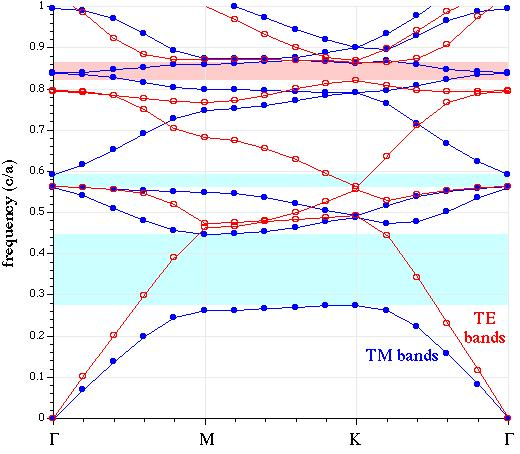
\includegraphics[width=5cm]{pics/test01_ref}}
    \subfigure[TE band diagram.]{\label{fig:test_1:TE}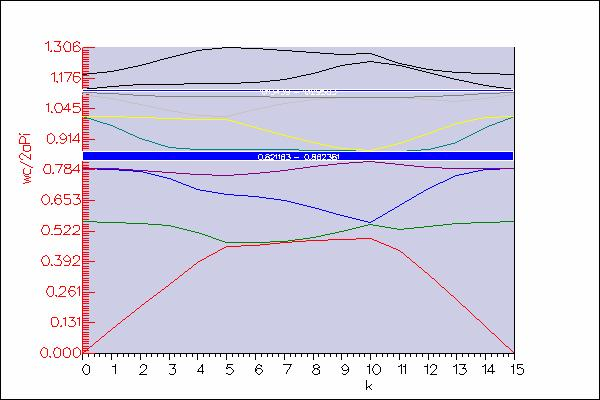
\includegraphics[width=5cm]{pics/test01_TE}}
    \subfigure[TM band diagram.]{\label{fig:test_1:TM}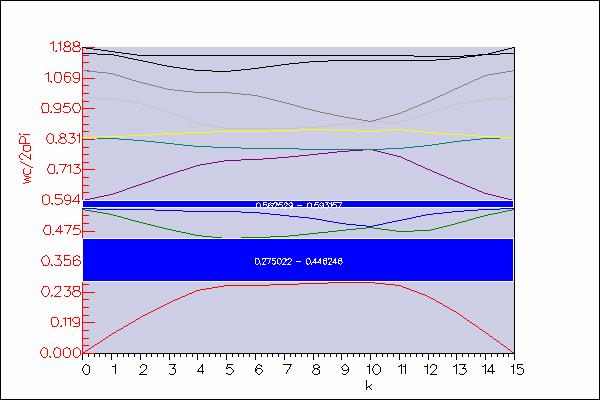
\includegraphics[width=5cm]{pics/test01_TM}}
    \subfigure[Real $H_z$ of the Bloch mode at k-point $M$, first band]{\label{fig:test_1:real}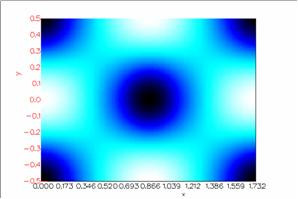
\includegraphics[width=5cm]{pics/test01_field_real}}
    \subfigure[Imag $H_z$ of the Bloch mode at k-point $M$, first band]{\label{fig:test_1:imag}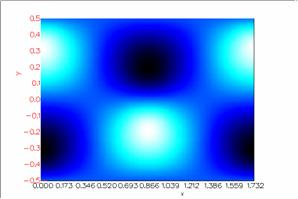
\includegraphics[width=5cm]{pics/test01_field_imag}}
  \end{center}
  \caption{Test 1.}
  \label{fig:test_1}
\end{figure}

\subsubsection{Test 2}

The structure considered in this test is a two-dimensional infinite
square lattice of dielectric rods in air
(\figref{fig:test_2:lattice}). The lattice vectors are:
\begin{equation*}
  \Vector{R}_1 = \left(1,0\right), \quad \Vector{R}_2 =
  \left(0,1\right)
\end{equation*}
The radius of the rods is $R = 0.2 \Lambda$, their refractive index is
$n_{cyl} = \sqrt{12}$.

\figref{fig:test_2:ref} shows the reference results: the figure is
taken from \cite{johnson_photonic}. The $k$-path studied is
$\Gamma-X-K-\Gamma$, in order to scan all the possible directions of
the irreducible Brillouin zone. No TE bandgaps are visible, while one
large TM bangap is present for $0.28 < F < 0.42$.

The results obtained with our implementation are reported in
\tabref{tab:test_2}, \figref{fig:test_2:TE} and \figref{fig:test_2:TM}, for TE and TM
polarization respectively. We can note the very good accordance with
reference results, within $1.2\%$. The small bandgaps in the TE
polarization are not ``real'', but only the consequence of the
discretization in the k-path.

\begin{table}[htbp]
  \begin{center}
    \subtable[TE polarization.]{
    \begin{tabular}{|*{5}{c|}}
      \hline
      Band & k-point & $F_{\text{our algorithm}}$ & $F_{\text{MPB}}$ & Error [$\%$] \\
      \hline
      1 & $\Gamma$ & 0 & 0 & 0 \\
        & $M$ & 0.413 & 0.42 & -0.7 \\
        & $K$ & 0.497 & 0.5 & -0.6 \\
      2 & $\Gamma$ & 0.55 & 0.565 & 1.2 \\
        & $M$ & 0.438 & 0.44 & 0.4 \\
        & $K$ & 0.586 & 0.59 & -0.7 \\
      3 & $\Gamma$ & 0.765 & 0.77 & -0.7 \\
        & $M$ & 0.636 & 0.64 & -0.6 \\
        & $K$ & 0.586 & 0.59 & -0.7 \\
      \hline
    \end{tabular}}
    \subtable[TM polarization.]{
    \begin{tabular}{|*{5}{c|}}
      \hline
      Band & k-point & $F_{\text{our algorithm}}$ & $F_{\text{MPB}}$ & Error [$\%$] \\
      \hline
      1 & $\Gamma$ & 0 & 0 & 0 \\
        & $M$ & 0.243 & 0.24 & 1.2 \\
        & $K$ & 0.281 & 0.28 & 0.4 \\
      2 & $\Gamma$ & 0.551 & 0.55 & 0.2 \\
        & $M$ & 0.417 & 0.42 & -0.7 \\
        & $K$ & 0.495 & 0.50 & -1.0 \\
      3 & $\Gamma$ & 0.552 & 0.55 & 0.4 \\
        & $M$ & 0.554 & 0.555 & -0.2 \\
        & $K$ & 0.495 & 0.50 & -1.0 \\
      \hline
    \end{tabular}}
  \end{center}
  \caption{TE and TM results. Note that the MPB results values have
    been extracted graphically from the available graph, so accuracy is
    not better that $0.01$. Overall accordance is within $1.2\%$.}
  \label{tab:test_2}
\end{table}

\figref{fig:test_2:real} and \figref{fig:test_2:imag} show the
$z$-component of the magnetic field of the Bloch mode for the TM
polarization at the $X$ k-point, at the first band.

\begin{figure}[htbp]
  \begin{center}
    \subfigure[Square lattice. In green, the fundamental cell.]{\label{fig:test_2:lattice}\resizebox{4cm}{!}{\input{pics/test02.pdf_t}}}
    \subfigure[Reference results from \cite{johnson_photonic}.]{\label{fig:test_2:ref}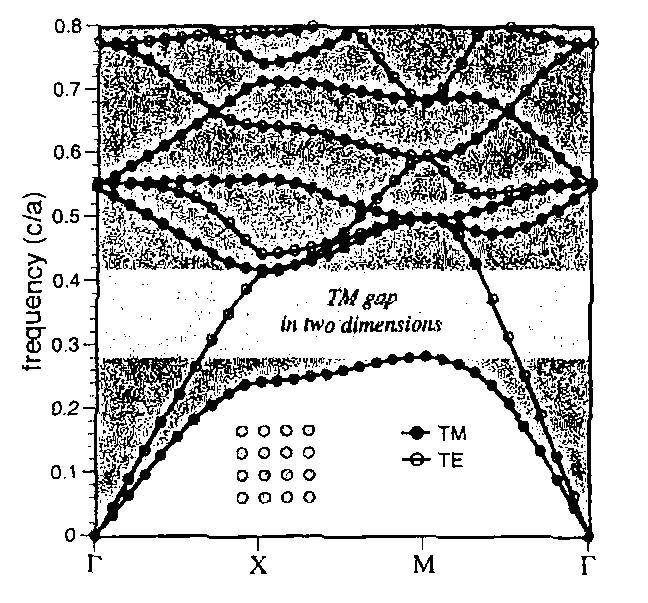
\includegraphics[width=5cm]{pics/test02_ref}}
    \subfigure[TE band diagram.]{\label{fig:test_2:TE}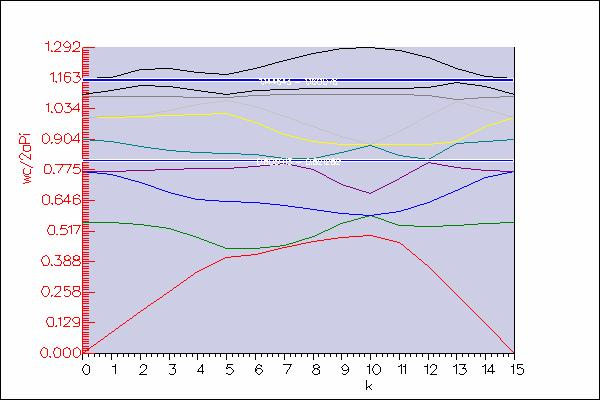
\includegraphics[width=5cm]{pics/test02_TE}}
    \subfigure[TM band diagram.]{\label{fig:test_2:TM}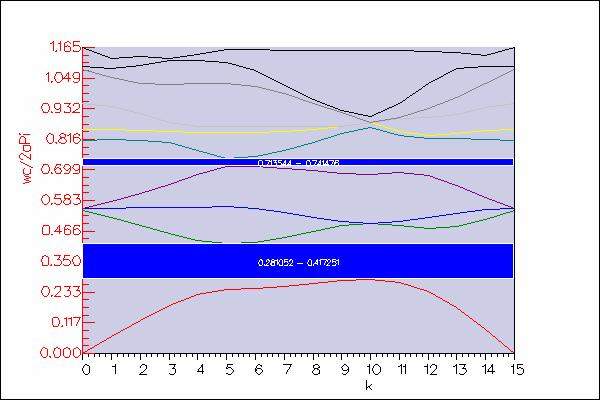
\includegraphics[width=5cm]{pics/test02_TM}}
    \subfigure[Real $H_z$ of the Bloch mode at k-point $X$, first band]{\label{fig:test_2:real}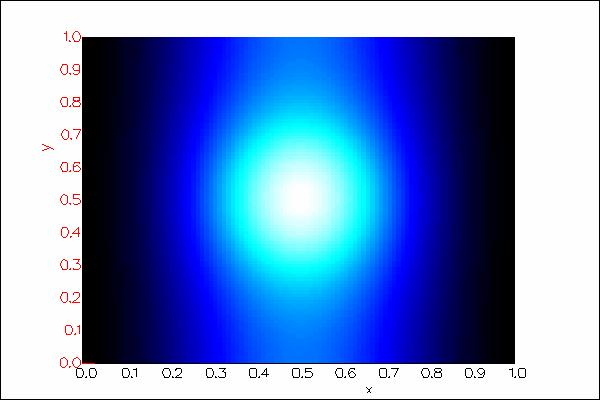
\includegraphics[width=5cm]{pics/test02_field_real}}
    \subfigure[Imag $H_z$ of the Bloch mode at k-point $X$, first band]{\label{fig:test_2:imag}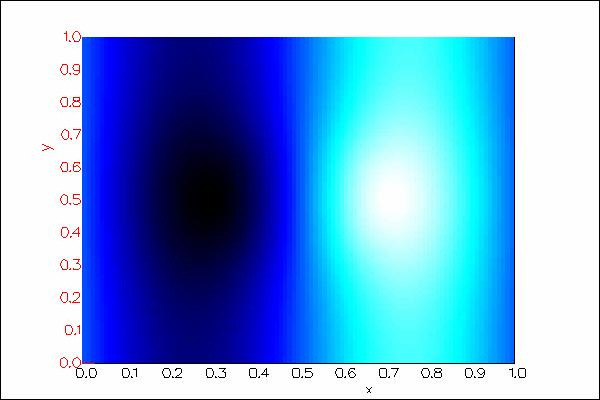
\includegraphics[width=5cm]{pics/test02_field_imag}}
  \end{center}
  \caption{Test 2.}
  \label{fig:test_2}
\end{figure}

\subsubsection{Test 3}

The structure considered in this test is a line defect in a two-dimensional 
triangular lattice of air holes in a dielectric substrate
(\figref{fig:test_3:lattice}). The lattice vectors are:
\begin{equation*}
  \Vector{R}_1 = \left( \frac{\sqrt{3}}{2}, -\frac{1}{2} \right),
  \quad \Vector{R}_2 = \left( \frac{\sqrt{3}}{2}, \frac{1}{2} \right)
\end{equation*}
The radius of the rods is $R = 0.309 \Lambda$, their refractive index is
$n_{sub} = 3.2$. Only the TE polarization is considered.

First, the bandgap of an infinite lattice, without defect, is
computed. Results are shown in \figref{fig:test_3:ref}, as computed by
CrystalWave, and \figref{fig:test_3:TE}, with our
algorithm. Numerical comparisons are given in \tabref{tab:test_3}.

\begin{table}[htbp]
  \begin{center}
    \begin{tabular}{|*{3}{c|}}
      \hline
      & First bandgap -- low $F$ & First bandgap -- high $F$ \\
      \hline
      Our algorithm & 0.226 & 0.289 \\
      CrystalWave & 0.221 & 0.281 \\
      \hline
    \end{tabular}
  \end{center}
  \caption{Comparison between our algorithm and CrystalWave, on the
  boundaries of the first bandgap for the TE polarization, for the
  complete lattice. Accordance is within $2\%$.}
  \label{tab:test_3}
\end{table}

CrystalWave algorithm consists in propagating a broadband
plane wave through the crystal, collect the result and inverse Fourier
transform it to get the spectral response of the device: it implicitely
studies just one direction of propagation through the crystal, the one
corresponding to the input planewave wavevector, that, in the example,
corresponds to $X$ k-point. This procedure is somehow limiting,
because in doesn't allow the user to study the full bandgap of the
structure: a lattice could, in fact, present a not-complete bandgap, i.e. a bandgap only for
certain directions, but non for all, and being misinterpreted for a
complete one. Our algorithm, on the other hand, scanning all the
directions of the irreducible Brillouin zone, avoids this problem and
gives a complete grasp of the device's bandgap.

 \figref{fig:test_3:ref} shows the power transmitted
through the device as a function of frequency. We can note a broad
range of frequencies for which the transmission is zero: this is a
bandgap in the direction of propagation of the input planewave. It
correspond to the first bandgap (shown in blue) in
\figref{fig:test_3:TE}.

\begin{figure}[htbp]
  \begin{center}
    \subfigure[Reference results computed by CrystalWave \cite{crystalwave}.]{\label{fig:test_3:ref}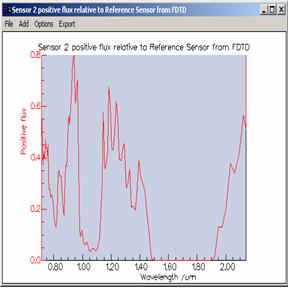
\includegraphics[width=5cm]{pics/test04_ref}}
    \subfigure[TE band diagram.]{\label{fig:test_3:TE}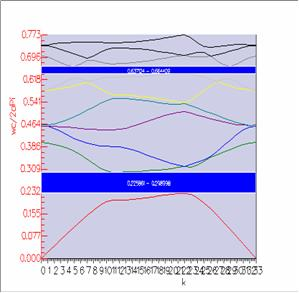
\includegraphics[width=5cm]{pics/test04_TE}}
  \end{center}
  \caption{Test 3: complete lattice.}
  \label{fig:test_3}
\end{figure}

With these informations, the line defect can now be studied. To model it, a supercell, as shown
in \figref{fig:test_3_line:lattice} in green, is taken and only the
directions parallel to the channel's axis are studied, i.e. the
wavevectors between $\Gamma$ and $X$. The results
obtained with our implementation are reported in
\figref{fig:test_3_line:TE}, and they have to be compared with
\figref{fig:test_3_line:ref}. Note that Crystalwave shows unitary
power for the frequencies inside the bandgap: they are guided
losslessy by the line defect through the crystal. The small deep at
the middle of the bandgap corresponds to the crossing point between
the even guided mode (whose characteristic has negative slope) and the
odd mode (whose characteristic has positive slope) in
\figref{fig:test_3_line:TE}. It is due to the fact that, for that
particular wavevector, the phase
velocity of the excited mode (which is the even mode, in CrystalWave)
is almost zero (i.e., its characteristic is almost flat): in a time-domain
algorithm as CrystalWave's, this means that power takes very long time to
get to the end of the device and to be computed. Lasting the
simulation longer would reduce the deep.

\begin{figure}[htbp]
  \begin{center}
    \subfigure[Line defect. In green, the super-cell.]{\label{fig:test_3_line:lattice}\resizebox{8cm}{!}{\input{pics/test04.pdf_t}}}
    \subfigure[Reference results computed by CrystalWave \cite{crystalwave}.]{\label{fig:test_3_line:ref}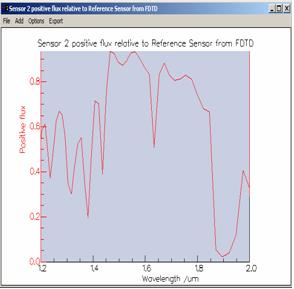
\includegraphics[width=5cm]{pics/test04_line_ref}}
    \subfigure[TE band diagram.]{\label{fig:test_3_line:TE}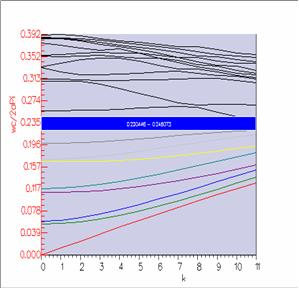
\includegraphics[width=5cm]{pics/test04_line_TE}}
    \subfigure[Real $H_z$.]{\label{fig:test_3_line:real}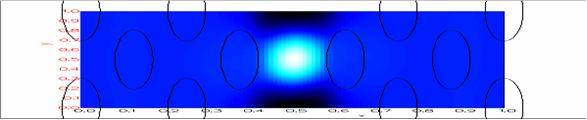
\includegraphics[width=5cm]{pics/test04_line_field_real}}
    \subfigure[Imag $H_z$.]{\label{fig:test_3_line:imag}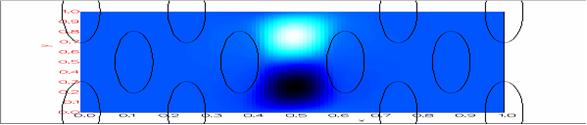
\includegraphics[width=5cm]{pics/test04_line_field_imag}}
  \end{center}
  \caption{Test 3: line defect.}
  \label{fig:test_3_line}
\end{figure}

The $z$-component of the magnetic field of the fundamental guided mode
is also shown in \figref{fig:test_3_line:real} and
\figref{fig:test_3_line:imag}, for the supercell.

\subsubsection{Test 4}

The structure considered in this test is a planar photonic crystal
waveguide, made of a triangular lattice of dielectric rods in air,
refractive index $n_{cil}^{high} = 3$ for a height $H = \Lambda$,
and refractive index $n_{cil}^{low} = 2$ infinitely above and below, radius
$R = 0.3 \Lambda$. See \figref{fig:test_4}.

\begin{figure}[htbp]
  \begin{center}
    \subfigure[Triangular lattice from \cite{johnson_photonic}.]{\label{fig:test_4:lattice}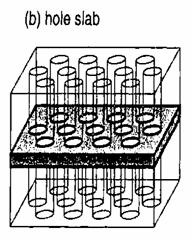
\includegraphics[width=5cm]{pics/test06}}
    \subfigure[Reference results from \cite{johnson_photonic}.]{\label{fig:test_4:ref}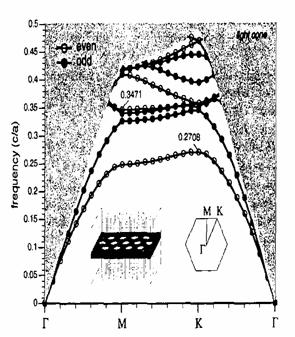
\includegraphics[width=5cm]{pics/test06_ref}}
    \subfigure[Band diagram.]{\label{fig:test_4:bands}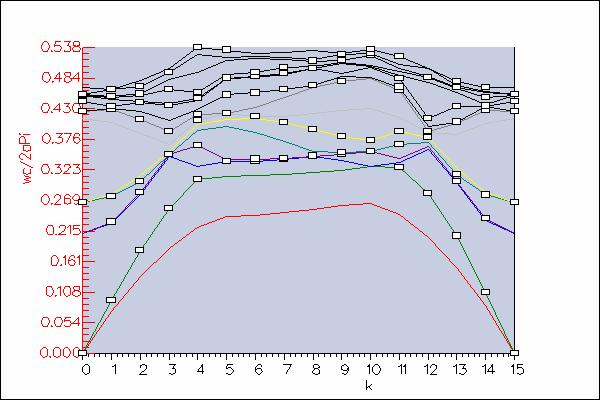
\includegraphics[width=5cm]{pics/test06_bands}}
  \end{center}
  \caption{Test 4.}
  \label{fig:test_4}
\end{figure}

\figref{fig:test_4:ref} shows the reference results and
\figref{fig:test_4:bands} the computed ones: \tabref{tab:test_4} shows
that the accordance is again very good.

\begin{table}[htbp]
  \begin{center}
    \begin{tabular}{|*{5}{c|}}
      \hline
      Band & k-point & $F_{\text{our algorithm}}$ & $F_{\text{MPB}}$ & Error [$\%$] \\
      \hline
      1 & $\Gamma$ & 0 & 0 & 0 \\
        & $M$ & 0.237 & 0.24 & -1.3 \\
        & $K$ & 0.268 & 0.27 & -0.7 \\
      2 & $\Gamma$ & 0 & 0 & 0 \\
        & $M$ & 0.312 & 0.32 & 2.6 \\
        & $K$ & 0.328 & 0.34 & -3.7 \\
      3 & $\Gamma$ & 0.215 & n/a & n/a \\
        & $M$ & 0.328 & 0.34 & -3.7 \\
        & $K$ & 0.328 & 0.34 & -3.7 \\
      \hline
    \end{tabular}
  \end{center}
  \caption{Comparison between the reference results and our
  algorithm's result. Overall accordance is within $3.7a\%$.}
  \label{tab:test_4}
\end{table}

As an example, \figref{fig:test_4_field} shows the profile of the real
part of the Bloch mode at the reciprocal lattice point $M$, first
band. The fields are plotted on an horizontal section passing through
the high index slab and on a vertical section passing through the
center of a unit cell

\begin{figure}[htbp]
  \begin{center}
    \subfigure[Horizontal section, $x$ component]{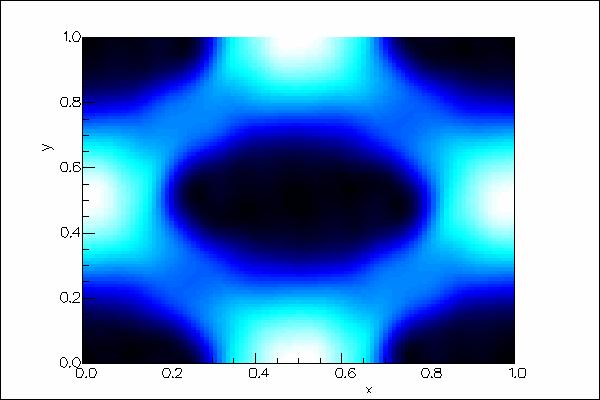
\includegraphics[width=5cm]{pics/test06_field_hor_x}}
    \subfigure[Horizontal section, $y$ component]{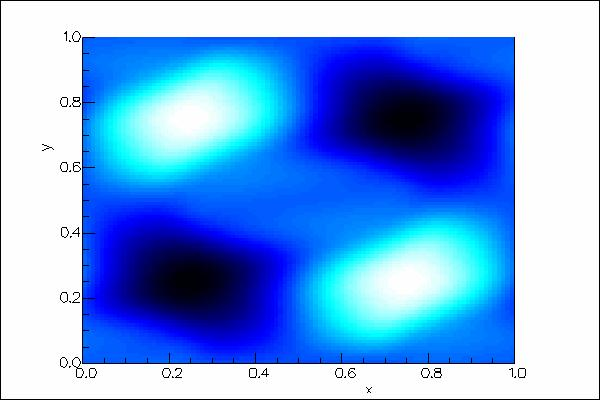
\includegraphics[width=5cm]{pics/test06_field_hor_y}}
    \subfigure[Vertical section, $x$ component]{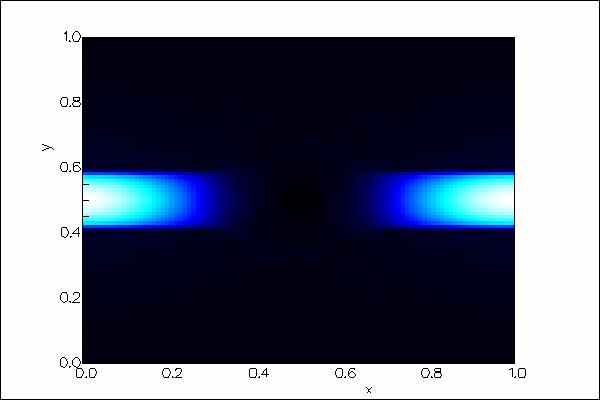
\includegraphics[width=5cm]{pics/test06_field_ver_x}}
    \subfigure[Vertical section, $y$ component]{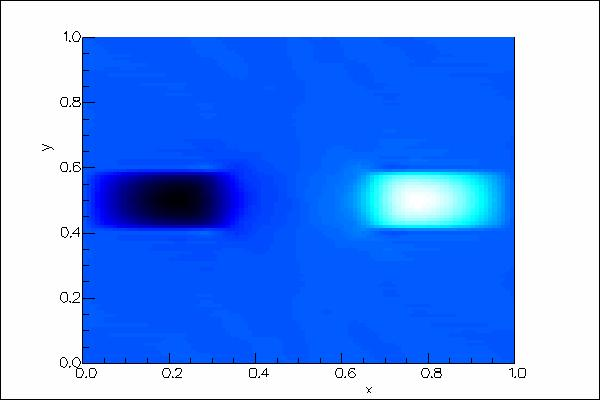
\includegraphics[width=5cm]{pics/test06_field_ver_y}}
  \end{center}
  \caption{Test 4: Real part of the Bloch mode, at k-point $M$, first
  band. Values on the axis are normalized to the lattice constant $\Lambda$.}
  \label{fig:test_4_field}
\end{figure}

